
%(BEGIN_QUESTION)
% Copyright 2011, Tony R. Kuphaldt, released under the Creative Commons Attribution License (v 1.0)
% This means you may do almost anything with this work of mine, so long as you give me proper credit

This Siemens S7-200 PLC is supposed to count the number of cars entering a parking garage, using a pressure-sensitive switch that the cars drive over when entering the garage.  The car-count value is sent to a computer in the main office via a network cable plugged into the PLC.  The parking attendant is able to reset the count to 0 at the end of his shift, using a key-switch:

$$\includegraphics[width=15.5cm]{i03683x01.eps}$$

Unfortunately, there is something wrong with this system.  Although it worked just fine yesterday, today the counter's current value as displayed on the main office computer seems to be stuck at 574 no matter how many more cars drive over the pressure switch and enter the garage.  Explain how you would go about diagnosing the problem in this system, justifying each step you would take.

\vskip 20pt \vbox{\hrule \hbox{\strut \vrule{} {\bf Suggestions for Socratic discussion} \vrule} \hrule}

\begin{itemize}
\item{} A useful troubleshooting strategy is to mentally divide this system into three major portions, and try to determine which portion the problem lies within: (1) the switches and wiring connected to the PLC, (2) the PLC itself, and (3) the network cable and computer in the main office.
\item{} How important is the fact that this system worked fine yesterday?  Does this knowledge help you in your troubleshooting?
\item{} Are there any LED indicators on the face of the PLC that might be helpful in providing diagnostic data for you to pinpoint the location of the problem?
\end{itemize}

\underbar{file i03683}
%(END_QUESTION)





%(BEGIN_ANSWER)


%(END_ANSWER)





%(BEGIN_NOTES)

You could try stepping on the pressure-sensitive switch and see if the corresponding input LED on the PLC ({\tt I0.1}) lights up.  If not, there's an I/O or wiring or switch failure.  If it does blink every time you step on the pressure switch, the problem lies within the PLC or else the HMI or the communications between them.

%INDEX% PLC, relating I/O status to virtual elements (troubleshooting)

%(END_NOTES)


